\section{电气元件}\label{sec:dianqiyuanjian}

{\bfseries 知识目标}
\begin{itemize}
\item 掌握图块的概念
\item 掌握图块的定义、插入、输出方法
\item 掌握图块属性定义与设置知识
\end{itemize}

{\bfseries 技能目标}
\begin{itemize}
\item 能够完成电子元件的定制
\end{itemize}

本任务以绘制\ref{fig:zhumodianlu}所示电路图中的电子元件为目标,主要是帮助读者掌握AutoCAD的图块的概念,以便于在绘图过程中将大量重复的图形定义为图块,以提高图形的绘制速度。

\subsection{电容元件}
首先,让我们来绘制图\ref{fig:zhumodianlu}所示电路图中的电容元件。

第一步,先绘制电容元件的对称中心线。

\noindent
\begin{figure}[htbp]
\centering
\subfloat[]{\label{fig:dianrong1}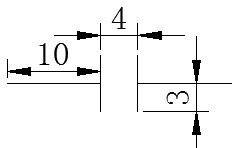
\includegraphics[scale=0.3]{dianrong1.png}}\hspace{20pt}
\subfloat[]{\label{fig:dianrong2}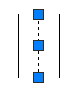
\includegraphics[scale=0.5]{dianrong2.png}}\hspace{20pt}
\subfloat[]{\label{fig:dianrong3}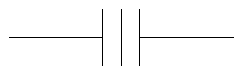
\includegraphics[scale=0.5]{dianrong3.png}}
\subfloat[]{\label{fig:dianrong4}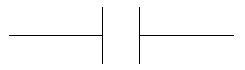
\includegraphics[scale=0.5]{dianrong4.png}}
\caption{电容元件绘制}
\end{figure}
\noindent

命令:line\\
指定第一点:\\
指定下一点或 [放弃(U)]: @6$<90$\\
指定下一点或 [放弃(U)]:\\
\indent

第二步,以对称中心做为偏移对象,向左右各偏移2mm,如图\ref{fig:dianrong2} 所示。

\noindent
命令: offset
当前设置: 删除源=否  图层=源  OFFSETGAPTYPE=0\\
指定偏移距离或 [通过(T)/删除(E)/图层(L)] $<$通过$>$:  2\\
选择要偏移的对象,或 [退出(E)/放弃(U)] $<$退出$>$:\\
指定要偏移的那一侧上的点,或 [退出(E)/多个(M)/放弃(U)] $<$退出$>$:\\
选择要偏移的对象,或 [退出(E)/放弃(U)] $<$退出$>$:\\
指定要偏移的那一侧上的点,或 [退出(E)/多个(M)/放弃(U)] $<$退出$>$:\\
选择要偏移的对象,或 [退出(E)/放弃(U)] $<$退出$>$:\\
\indent

第三步,绘电容接线时,以其最左侧竖线的中心点为起点向左绘制10mm的线条,然后以中心线做另一电容接线,最终结果如图\ref{fig:dianrong3}所示。

\noindent
命令: line\\
指定第一点: mid\\
于\\
指定下一点或 [放弃(U)]: @10$<$-180\\
指定下一点或 [放弃(U)]:\\
命令: mirror\\
选择对象: 找到 1 个\\
选择对象:  指定镜像线的第一点: 指定镜像线的第二点:\\
要删除源对象吗?[是(Y)/否(N)] $<N>:$

\indent
最后,删除中心线,完成电容元件的绘制,其结果如图\ref{fig:dianrong4}所示。

由于电器元件通常都需要重复使用,为提高绘图速度,我们需要将绘制的电气元件定义为块并写入文件中,才能够实现其重复利用的目的。下面我们将通过电容块的定义来说明块的定义过程。当我们输入block命令后,会出现图\ref{fig:kuaidingyi}所示的块定义窗体。我们在窗体中命名块的名称为电容,点击拾取点并选择电容元件的最左点来完成基点的定义,点击选择对象并选整个电容图形来完成对象的定义,最后点击确定。

\noindent
命令: block 指定插入基点:\\
选择对象: 指定对角点: 找到 4 个\\
选择对象:\\

\indent
完成块定义后,还需要通过块写命令wblock将定义的块写入dwg文件中才能够实现随时调用和重复利用。输入wblock命令后,会出现图\ref{fig:kuaixie}所示对话框,选择块并选择好块文件保存的路径即可完成块写操作。当块写为文件后就可以在新的CAD文件中调用,真正实现一处定义多处使用,提高绘图效率。

\noindent
\begin{figure}[htbp]
\centering
\begin{floatrow}
\ffigbox{\caption{块定义}\label{fig:kuaidingyi}}{
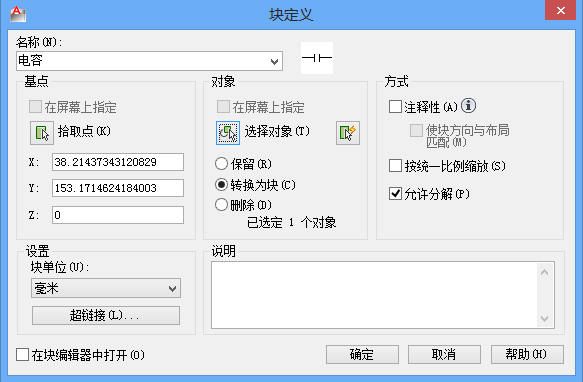
\includegraphics[scale=0.4]{kuaidingyi.png}
}
\ffigbox{\caption{块写}\label{fig:kuaixie}}{
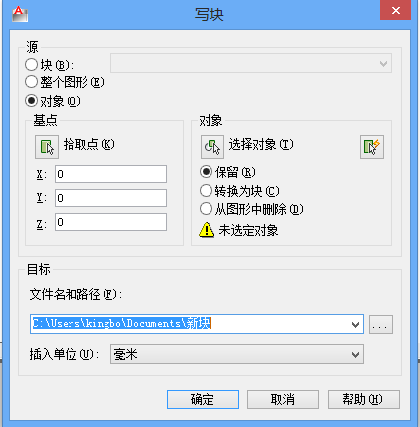
\includegraphics[scale=0.35]{kuaixie.png}
}
\end{floatrow}
\end{figure}
\indent

\subsection{接地元件}
接地元件的绘制比较简单,先绘制一根做为基础,接下来通过偏移得到另外两根,通过缩放将偏移得两的线调整为相应的长度即可,并最长的一根上绘制连接线,然后将其定义为块并写入文件,如图\ref{fig:jiedi}所示。

\noindent
\begin{figure}[htbp]
\centering
\subfloat[]{\label{fig:jiedicicu}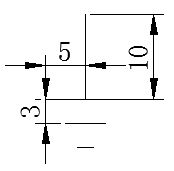
\includegraphics[scale=0.6]{jiedicicun.png}}\hspace{30pt}
\subfloat[]{\label{fig:jiedi1}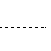
\includegraphics[scale=1]{suofang.png}}\hspace{30pt}
\subfloat[]{\label{fig:jiedi}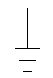
\includegraphics[scale=1]{jiedixian.png}}
\caption{接地元件绘制}
\end{figure}

\noindent
命令: line \\
指定第一点:\\
指定下一点或 [放弃(U)]: $@6<0$\\
指定下一点或 [放弃(U)]:\\
命令: offset\\
当前设置: 删除源=否  图层=源  OFFSETGAPTYPE=0\\
指定偏移距离或 [通过(T)/删除(E)/图层(L)] $<$通过$>$:  3\\
选择要偏移的对象,或 [退出(E)/放弃(U)]$<$退出$>$:\\
指定要偏移的那一侧上的点,或 [退出(E)/多个(M)/放弃(U)]$<$退出$>$:\\
选择要偏移的对象,或 [退出(E)/放弃(U)] $<$退出$>$:\\
指定要偏移的那一侧上的点,或 [退出(E)/多个(M)/放弃(U)]$<$退出$>$:\\
选择要偏移的对象,或 [退出(E)/放弃(U)] $<$退出$>$:\\
令: scale\\
选择对象: 找到 1 个\\
选择对象:\\
指定基点: mid\\
于\\
指定比例因子或 [复制(C)/参照(R)]: r\\
指定参照长度 $<$1.0000$>$: 10\\
指定新的长度或 [点(P)] $<$1.0000$>$:  5\\
令: scale\\
选择对象: 找到 1 个\\
选择对象:\\
指定基点: mid\\
于\\
指定比例因子或 [复制(C)/参照(R)]: r\\
指定参照长度 $<$10.0000$>$: 10\\
指定新的长度或 [点(P)]$ <5.0000>$:  2\\
命令: line \\
指定第一点: mid\\
于\\
指定下一点或 [放弃(U)]: $@10<90$\\
指定下一点或 [放弃(U)]:\\
\indent
\subsection{电阻元件}
电阻元件的绘制方法是:先绘制一个长10宽4的矩形,然后再绘制两根长10的直线,具体尺寸和结果如图\ref{fig:dianzucicu}和\ref{fig:dianzu}所示。

\noindent
\begin{figure}[htbp]
\centering
\subfloat[]{\label{fig:dianzucicu}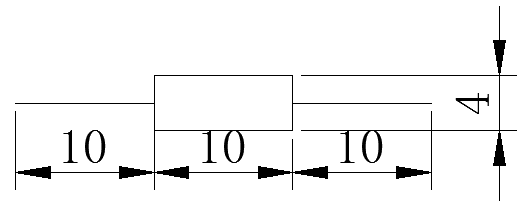
\includegraphics[scale=0.4]{dianzucichun.png}}\hspace{30pt}
\subfloat[]{\label{fig:dianzu}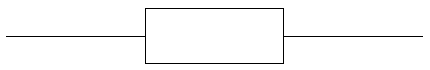
\includegraphics[scale=0.5]{dianzu.png}}
\caption{电阻元件绘制}
\end{figure}

\noindent
命令: rectang\\
指定第一个角点或 [倒角(C)/标高(E)/圆角(F)/厚度(T)/宽度(W)]:0,0\\
指定另一个角点或 [面积(A)/尺寸(D)/旋转(R)]: @10,4\\
命令:line 指定第一点: mid\\
于\\
指定下一点或 [放弃(U)]:$ @10<180$\\
指定下一点或 [放弃(U)]:\\
命令: mirror\\
选择对象: 找到 1 个\\
选择对象:  指定镜像线的第一点: mid\\
于 指定镜像线的第二点: mid\\
于\\
要删除源对象吗?[是(Y)/否(N)] $<N>:$\\

\subsection{电灯元件}
电灯元件的绘制过程:先绘制圆,接下来将其等分为8等分,然后绘制两条相交直线,最后绘制电源连接线即可。电灯元件的具体尺寸和结果如图\ref{fig:diandengcicu}和\ref{fig:diandeng3}所示。

\noindent
\begin{figure}[htbp]
\centering
\subfloat[]{\label{fig:diandengcicu}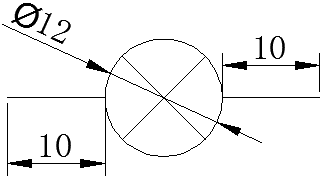
\includegraphics[scale=0.3]{diandeng.png}}\hspace{30pt}
\subfloat[]{\label{fig:diandeng1}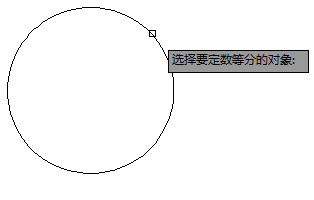
\includegraphics[scale=0.3]{diandeng1.png}}\hspace{30pt}
\subfloat[]{\label{fig:diandeng2}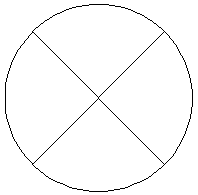
\includegraphics[scale=0.3]{diandeng2.png}}\hspace{30pt}
\subfloat[]{\label{fig:diandeng3}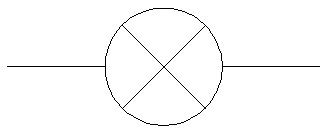
\includegraphics[scale=0.4]{diandeng3.png}}
\caption{电灯元件绘制}
\end{figure}

\noindent
命令: circle\\
 指定圆的圆心或 [三点(3P)/两点(2P)/切点、切点、半径(T)]:
指定圆的半径或 [直径(D)]: 6\\
命令: divide\\
选择要定数等分的对象:\\
输入线段数目或 [块(B)]: 8\\
命令: line 指定第一点: node\\
于\\
指定下一点或 [放弃(U)]: node\\
于\\
指定下一点或 [放弃(U)]:\\
命令:  LINE 指定第一点: node\\
于\\
指定下一点或 [放弃(U)]: node\\
于\\
命令: line\\
指定第一点: node\\
于\\
指定下一点或 [放弃(U)]: $@10<0$\\
指定下一点或 [放弃(U)]:\\
命令: mirror\\
选择对象: 找到 1 个\\
选择对象:  指定镜像线的第一点: node\\
于\\
指定镜像线的第二点: node\\
于\\
要删除源对象吗?[是(Y)/否(N)] $<N>:$
\subsection{二极管元件}
二极元件绘制过程:先绘制等边三角形,再绘制截止线,最后绘制电线。具体尺寸和结果如图所示。

\noindent
\begin{figure}[htbp]
\centering
\subfloat[]{\label{fig:erjiguancicu}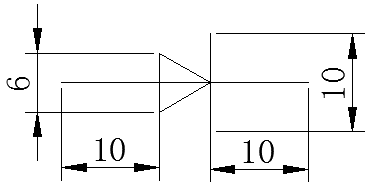
\includegraphics[scale=0.6]{erjiguancicu.png}}\hspace{30pt}
\subfloat[]{\label{fig:erjiguan}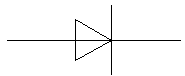
\includegraphics[scale=1]{erjiguan1.png}}
\caption{二极管元件绘制}
\end{figure}

\noindent
命令:polygon 输入侧面数$ <4>$:3
指定正多边形的中心点或 [边(E)]: e
指定边的第一个端点:0,0
指定边的第二个端点: $@6<270$
命令: line \\
指定第一点: mid\\
于\\
指定下一点或 [放弃(U)]: $@10<180$\\
指定下一点或 [放弃(U)]:\\
命令: line \\
指定第一点:end\\
于\\
指定下一点或 [放弃(U)]:end\\
于\\
指定下一点或 [放弃(U)]:$ @5<90$\\
指定下一点或 [闭合(C)/放弃(U)]:\\
命令:  LINE \\
指定第一点:end\\
于\\
指定下一点或 [放弃(U)]: $@5<-90$\\
指定下一点或 [放弃(U)]:\\
命令: line\\
指定第一点:end\\
指定下一点或 [放弃(U)]: $@10<0$\\
指定下一点或 [放弃(U)]:\\

\subsection{三极管元件}
三极管元件绘制过程:先绘一等边三角形,接下来将一这进行偏移,进行修剪得到内部结构,再用pline绘制箭头,最后绘制边接线。其尺寸及结果如图所示。

\noindent
\begin{figure}[htbp]
\centering
\subfloat[]{\label{fig:sanjiguancicu}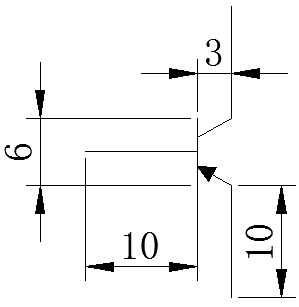
\includegraphics[scale=0.4]{sanjiguancicu.png}}\hspace{30pt}
\subfloat[]{\label{fig:sanjiguanPNP}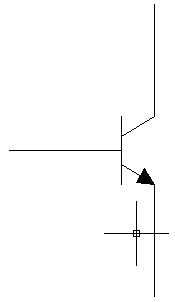
\includegraphics[scale=0.4]{sanjiguanPNP.png}}\hspace{30pt}
\subfloat[]{\label{fig:sanjiguanNPN}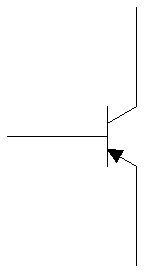
\includegraphics[scale=0.4]{sanjiguanNPN.png}}
\caption{三极管元件绘制}
\end{figure}

\noindent
命令: polygon \\
输入侧面数 $<3>$:\\
指定正多边形的中心点或 [边(E)]: e\\
指定边的第一个端点:0,0\\
指定边的第二个端点: $@6<-30$\\
命令: explode\\
选择对象: 找到 1 个\\
选择对象:\\
命令: offset\\
当前设置: 删除源=否  图层=源  OFFSETGAPTYPE=0
指定偏移距离或 [通过(T)/删除(E)/图层(L)] $<$通过$>$: 3\\
选择要偏移的对象,或 [退出(E)/放弃(U)] $<$退出$>$:\\
指定要偏移的那一侧上的点,或 [退出(E)/多个(M)/放弃(U)] $<$退出$>$:\\
选择要偏移的对象,或 [退出(E)/放弃(U)] $<$退出$>$:\\
命令: trim\\
当前设置:投影=UCS,边=无\\
选择剪切边...\\
选择对象或 $<$全部选择$>$:  找到 1 个
选择对象:
选择要修剪的对象,或按住 Shift 键选择要延伸的对象,或
[栏选(F)/窗交(C)/投影(P)/边(E)/删除(R)/放弃(U)]:\\
选择要修剪的对象,或按住 Shift 键选择要延伸的对象,或
[栏选(F)/窗交(C)/投影(P)/边(E)/删除(R)/放弃(U)]:\\
选择要修剪的对象,或按住 Shift 键选择要延伸的对象,或
[栏选(F)/窗交(C)/投影(P)/边(E)/删除(R)/放弃(U)]:\\
命令: erase 找到 1 个\\
命令: line 指定第一点: mid\\
于
指定下一点或 [放弃(U)]: $@10<180$\\
指定下一点或 [放弃(U)]:\\
命令: line\\
指定第一点: end\\
于\\
指定下一点或 [放弃(U)]:$ @10<90$\\
指定下一点或 [放弃(U)]:\\
命令: line\\
指定第一点:end\\
指定下一点或 [放弃(U)]:$ @10<-90$
指定下一点或 [放弃(U)]:\\
命令: PLINE
指定起点:end\\
当前线宽为 0.0000\\
指定下一个点或 [圆弧(A)/半宽(H)/长度(L)/放弃(U)/宽度(W)]: w\\
指定起点宽度$ <$0.0000$>$:
指定端点宽度 $<$0.0000$>$: 1.5
指定下一个点或 [圆弧(A)/半宽(H)/长度(L)/放弃(U)/宽度(W)]:$ @1.5<150$
指定下一点或 [圆弧(A)/闭合(C)/半宽(H)/长度(L)/放弃(U)/宽度(W)]:\\

\section{触摸延时开关电路图}
\endinput